\input{Preamble.tex}

\usepackage{float}
\usepackage[caption = false]{subfig}


\begin{document}

%%%%%%%%%%%%%%%%%%%%%%%%%%%%%%%%%%%%%%%%%%%%%%%%%%%%%%%%%%%%%%%%%%%%%%%%% 
%								CARATULA								%
%%%%%%%%%%%%%%%%%%%%%%%%%%%%%%%%%%%%%%%%%%%%%%%%%%%%%%%%%%%%%%%%%%%%%%%%% 

\begin{titlepage}

\newcommand{\HRule}{\rule{\linewidth}{0.5mm}}
\center
\mbox{\textsc{\large \bfseries {INSTITUTO TECNOLÓGICO DE BUENOS AIRES}}}\\[1cm]
\textsc{\Large 22.42 Laboratorio de Electrónica}\\[0.5cm]


\HRule \\[0.6cm]
{ \Huge \bfseries Trabajo Práctico N$^{\circ}$4}\\[0.4cm] 
\HRule \\[1.5cm]


{\large

\emph{Grupo 3}\\
\vspace{3px}

\begin{tabular}{lr} 	
\textsc{Bertachini}, Germán  & 58750 \\ 	
\textsc{Lambertucci}, Guido Enrique  & 58009 \\
\textsc{Londero Bonaparte}, Tomás Guillermo  & 58150 \\
\textsc{Mechoulam}, Alan  &  58438\\
\textsc{Scapolla}, Franco & 58465
\end{tabular}

\vspace{20px}

\emph{Profesores}\\
\vspace{3px}
\textsc{Cossutta}, Pablo Martín\\
\textsc{Weill}, María\\
\textsc{Salvati}, Matías\\	
\vspace{100px}

\begin{tabular}{ll}

Presentado: & 15/10/19\\

\end{tabular}

}

\vfill

\end{titlepage}



%%%%%%%%%%%%%%%%%%%%%%%%%%%%%%%%%%%%%%%%%%%%%%%%%%%%%%%%%%%%%%%%%%%%%%%%% 
%								INFORME									%
%%%%%%%%%%%%%%%%%%%%%%%%%%%%%%%%%%%%%%%%%%%%%%%%%%%%%%%%%%%%%%%%%%%%%%%%%



\section{Introducción}
El circuito presentado para la medición corresponde al de una fuente conmutada como se observa en la figura ()
\begin{figure}[H]
	\centering
	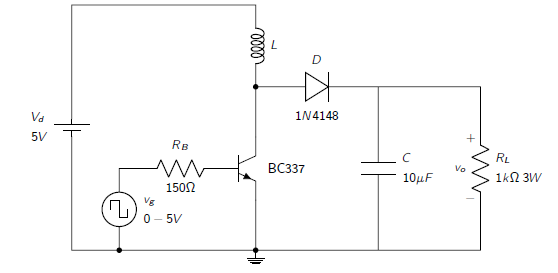
\includegraphics[width=0.9\textwidth]{Imagenes/circ.png}
\caption{Circuito fuente conmutada.}
	\label{fig:fcon}
\end{figure}

\section{Desarrollo de la experiencia}
Lo primero que se hizo fue exitar el circuito con una onda cuadrada de 0 a 5 volts, barriendo en frecuencias de 2kHz ~ 200kHz.
Se observó comparando la entrada con la salida que el circuito tiende a rectificar la señal e amplificarla, dependiendo la frecuencia amplificará mas o menos la señal, comenzando en un máximo local, que en estas condiciones coincide con el máximo absoluto, luego llegando a un mínimo local, para crecer nuevamente en el rango de frecuencias en el que se trabajó.\\
A continuación veremos algunas capturas de los puntos relevantes, siendo estos la frecuencia de inicio, la frecuencia del mínimo local, y la frecuencia final.

\begin{figure}[H]
	\centering
	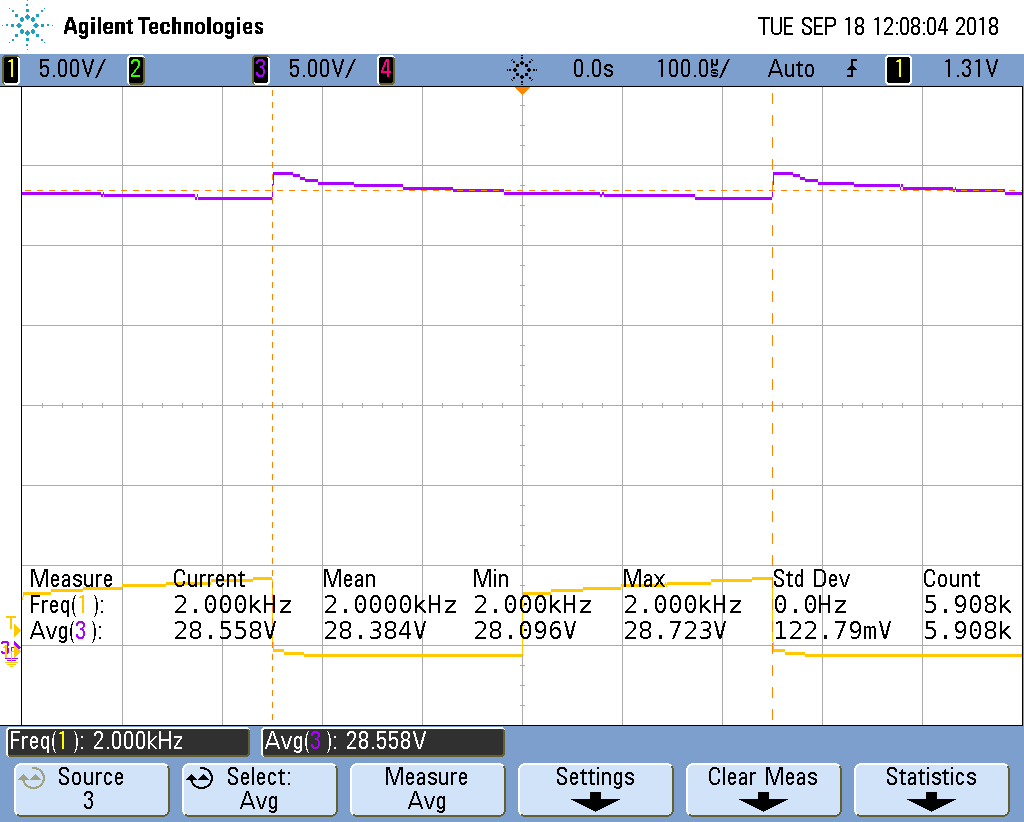
\includegraphics[width=0.9\textwidth]{Imagenes/tp3_labo3.png}
\caption{Fuente conmutada, frecuencia inicial [2kHz].}
	\label{fig:fcon}
\end{figure}

\begin{figure}[H]
	\centering
	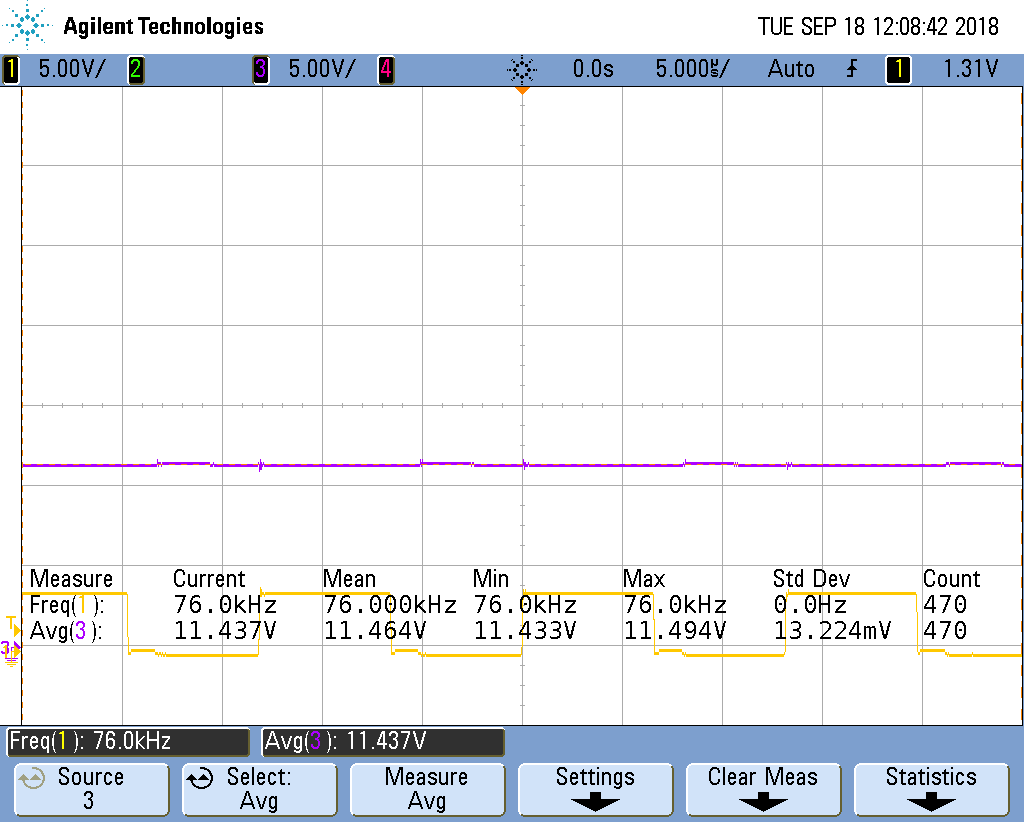
\includegraphics[width=0.9\textwidth]{Imagenes/tp3_labo4.png}
\caption{Fuente conmutada, frecuencia mínimo [76kHz].}
	\label{fig:fcon}
\end{figure}

\begin{figure}[H]
	\centering
	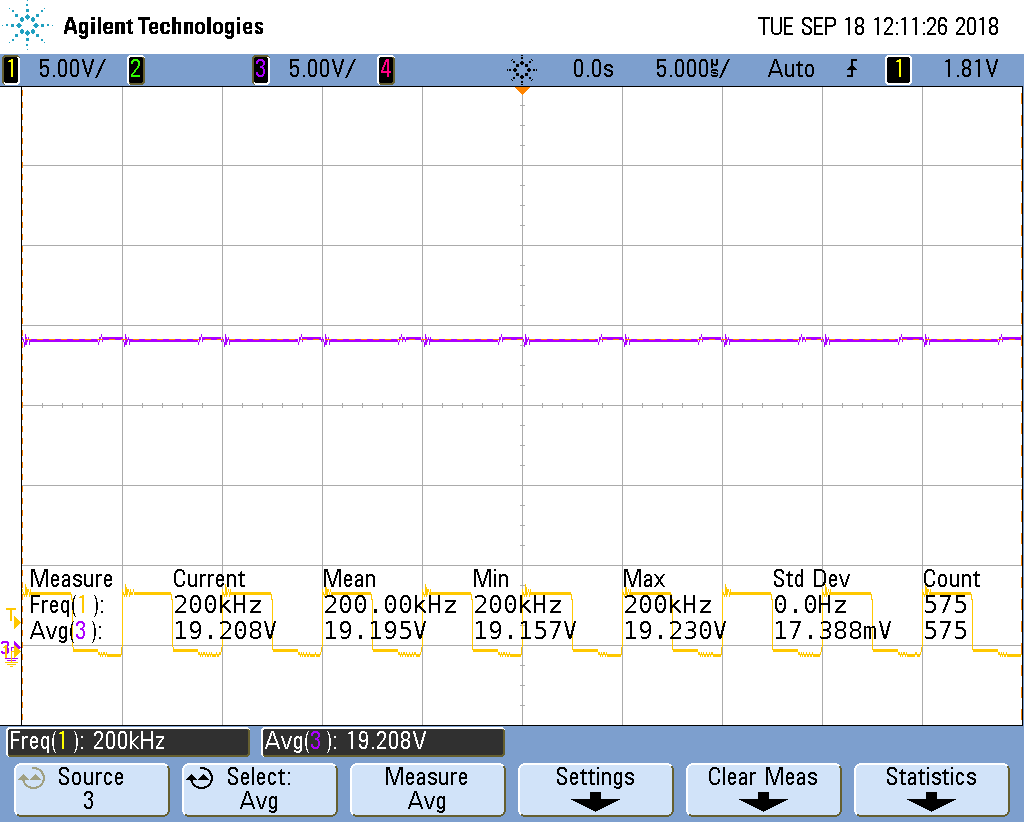
\includegraphics[width=0.9\textwidth]{Imagenes/tp3_labo5.png}
\caption{Fuente conmutada, frecuencia final [200kHz].}
	\label{fig:fcon}
\end{figure}
 
Luego, se procedió a alterar el Duty-Cycle de la señal de entrada, asi efectivamente modificando su pontencia, con una fecuencia fija de 25kHz.
A medida que se cambia el Duty-Cycle, su potencia varía , aumenta la tensión de salida  (en el caso de que se aumente la potencia) y disminuye en caso de bajarla.
\begin{figure}[H]
	\centering
	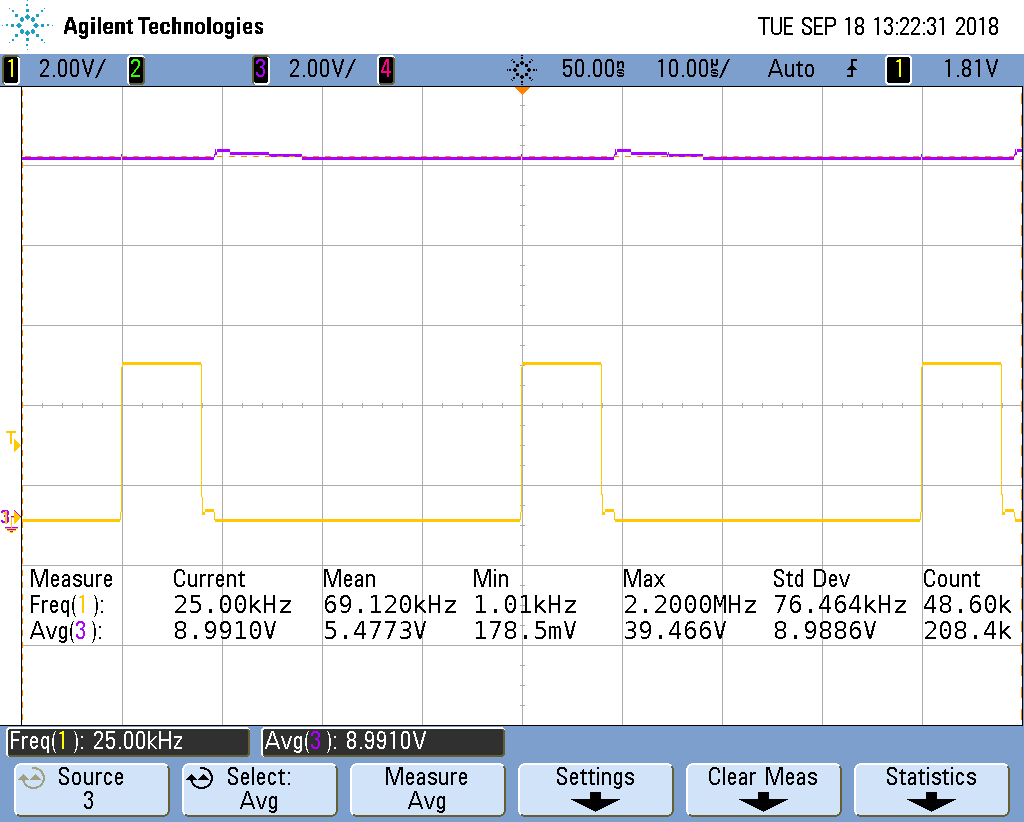
\includegraphics[width=0.9\textwidth]{Imagenes/dc_20.png}
\caption{Fuente conmutada, Duty-Cycle [20\%].}
	\label{fig:fcon}
\end{figure}
\begin{figure}[H]
	\centering
	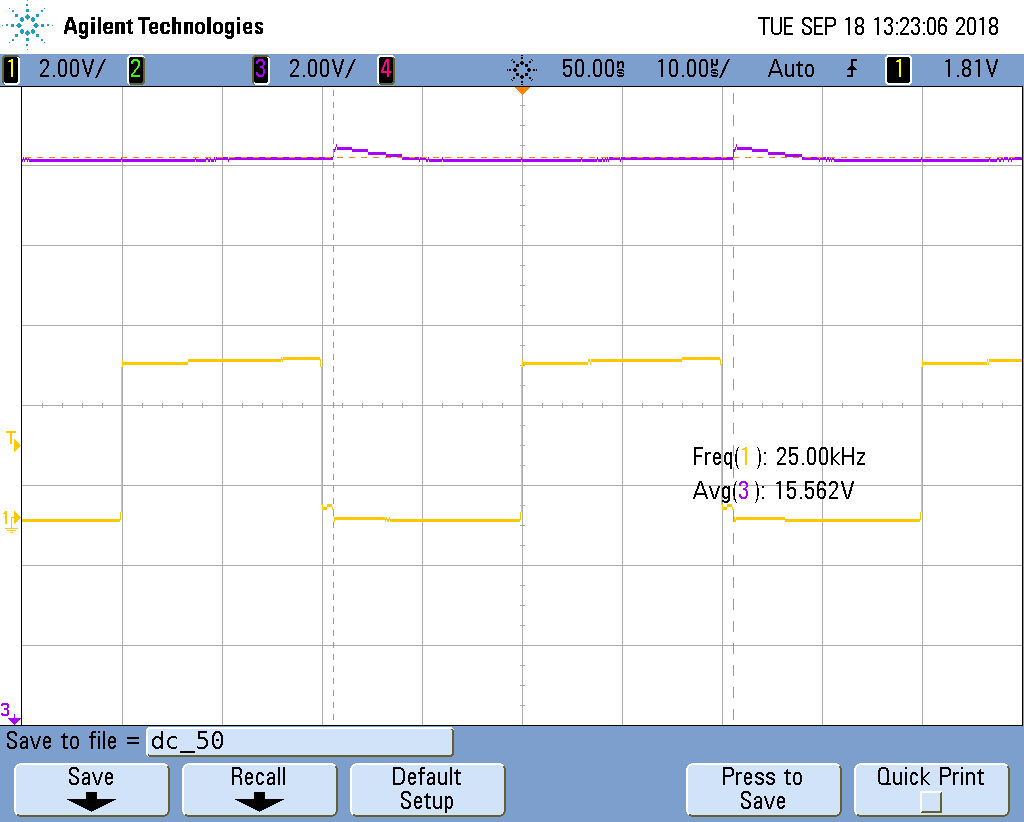
\includegraphics[width=0.9\textwidth]{Imagenes/dc_50.png}
\caption{Fuente conmutada, Duty-Cycle [50\%].}
	\label{fig:fcon}
\end{figure} 
\begin{figure}[H]
	\centering
	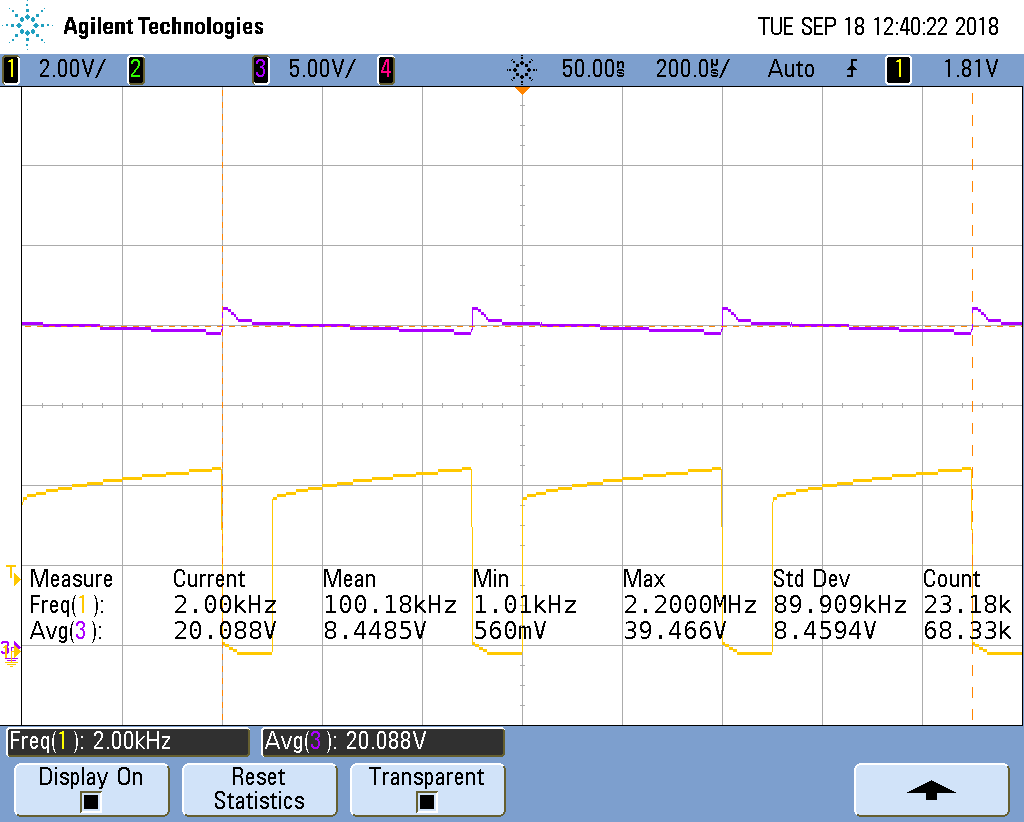
\includegraphics[width=0.9\textwidth]{Imagenes/dc_80.png}
\caption{Fuente conmutada, Duty-Cycle [80\%].}
	\label{fig:fcon}
\end{figure}
Para analizar la dependendencia de la ganancia con el Duty-Cycle se notó que a medida que aumenta el Duty-Cycle aumenta la ganancia, por lo cual inicialmente se propuso una dependencia lineal de la forma:
\begin{align}G = \frac{V_o}{V_i} = D \end{align}
Dado a que no coincidiía con loa realidad se descartó y se propuso la siguiente dependencia:
\begin{align}G = \frac{V_o}{V_i} = \frac{1}{1-D} \end{align}
La cual se adapta mucho mejor a las mediciones.\\
Se continuó por medir la respuesta al escalón del circuito en condiciones nominales obteniendo el siguiente gráfico:
\begin{figure}[H]
	\centering
	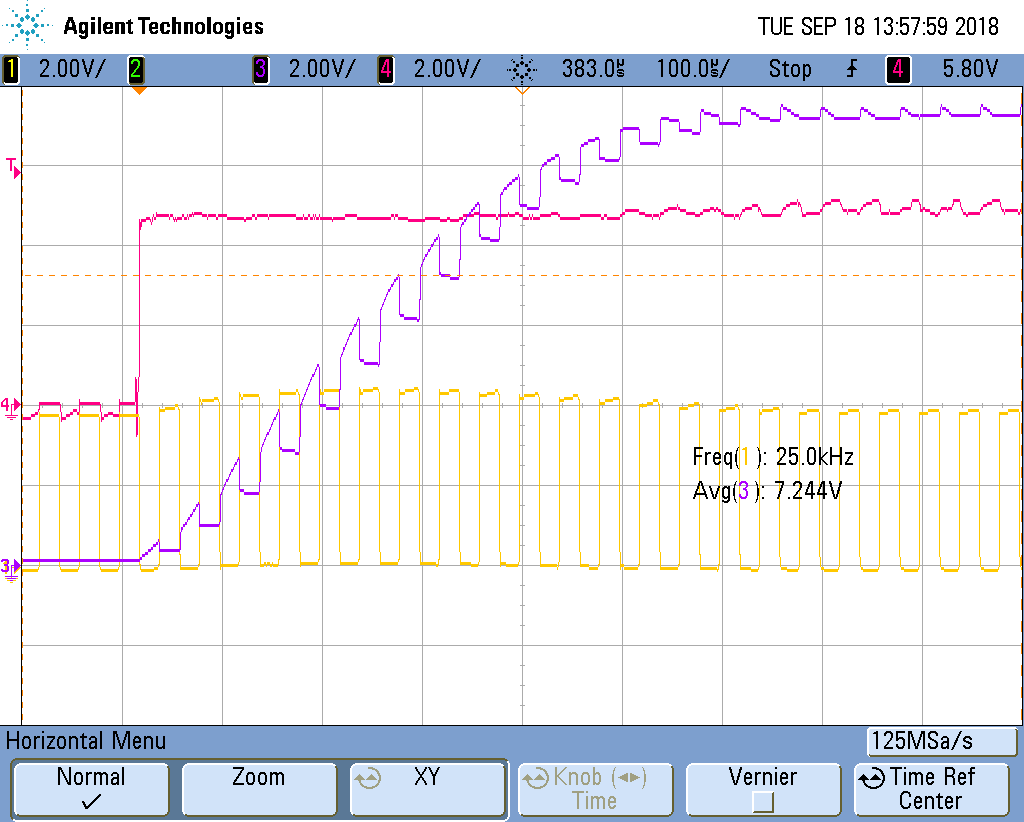
\includegraphics[width=0.9\textwidth]{Imagenes/sr.png}
\caption{Fuente conmutada,Respuesta al Escalón.}
	\label{fig:fcon}
\end{figure}
Se observa la variación de los picos en la salida, que a medida que se establece la señal, los picos decrecen en tamaño. Que los ciclos de estos picos coinciden con los de la cuadrada de entrada.\\
Luego se midió el ripple de salida del circuito, utilizando una frecuencia de entrada de 25kHz. Se observó que cuanto al agregar un capacitor en paralelo, y asi aumentando la componente capacitiva de la impedancia, decrece el sobrepico del ripple.\\Esto se puede también pensar como, dado a que una de las funciones del capacitor es mantener la tensión una función continua, cuando la tensión tiende a ser no continua, el capacitor lo suaviza, cuanto mas alta sea la capacidad mayor será su efecto de suavizamiento sobre la tensión.
\begin{figure}[H]
	\centering
	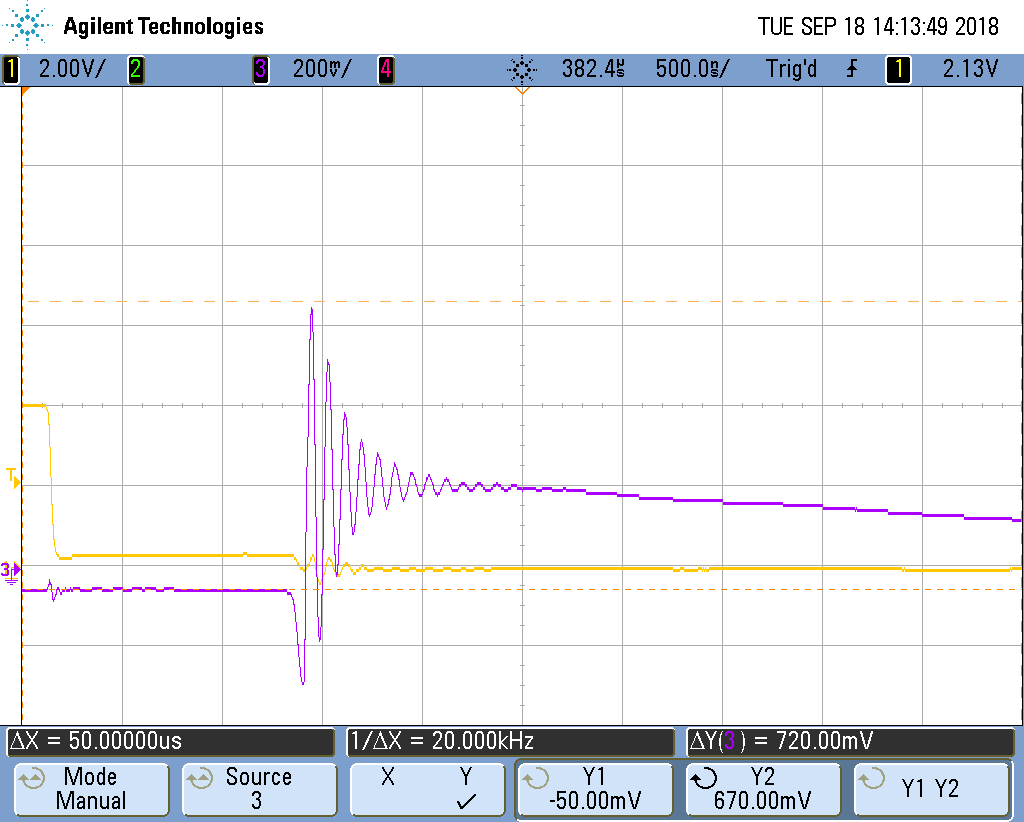
\includegraphics[width=0.9\textwidth]{Imagenes/ripple_.png}
\caption{Tensión de ripple de la salida de la Fuente conmutada.}
	\label{fig:fconr}
\end{figure}
\begin{figure}[H]
	\centering
	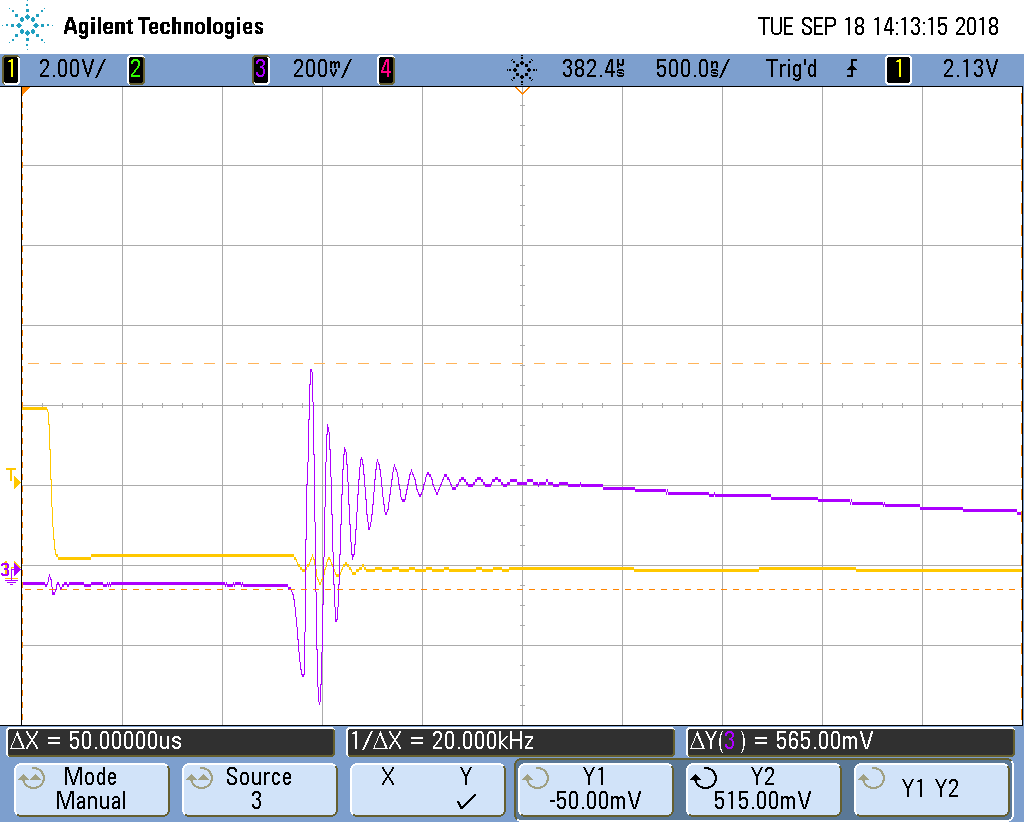
\includegraphics[width=0.9\textwidth]{Imagenes/ripple_c.png}
\caption{Tensión de ripple de la salida de la Fuente conmutada introduciendo un capacitor.}
	\label{fig:fconrc}
\end{figure}

Se continuó por medir la tensión en la bobina, esto se hizo al poner una punta de osciloscopio en cada terminal de la bobina y usar la función de Math '-' para obtener la tensión deseada.Para obtener la corriente se tuvo que usar la función interna de math utilizando el operador '-' para obtener la tensión sobre la bobina y luego mostrando la función al integrarla, dado que la bobina cumple la relación:
\begin{align} V_{coil} = L \cdot \frac{dI_{coil}}{dt}\end{align}
\begin{figure}[H]
	\centering
	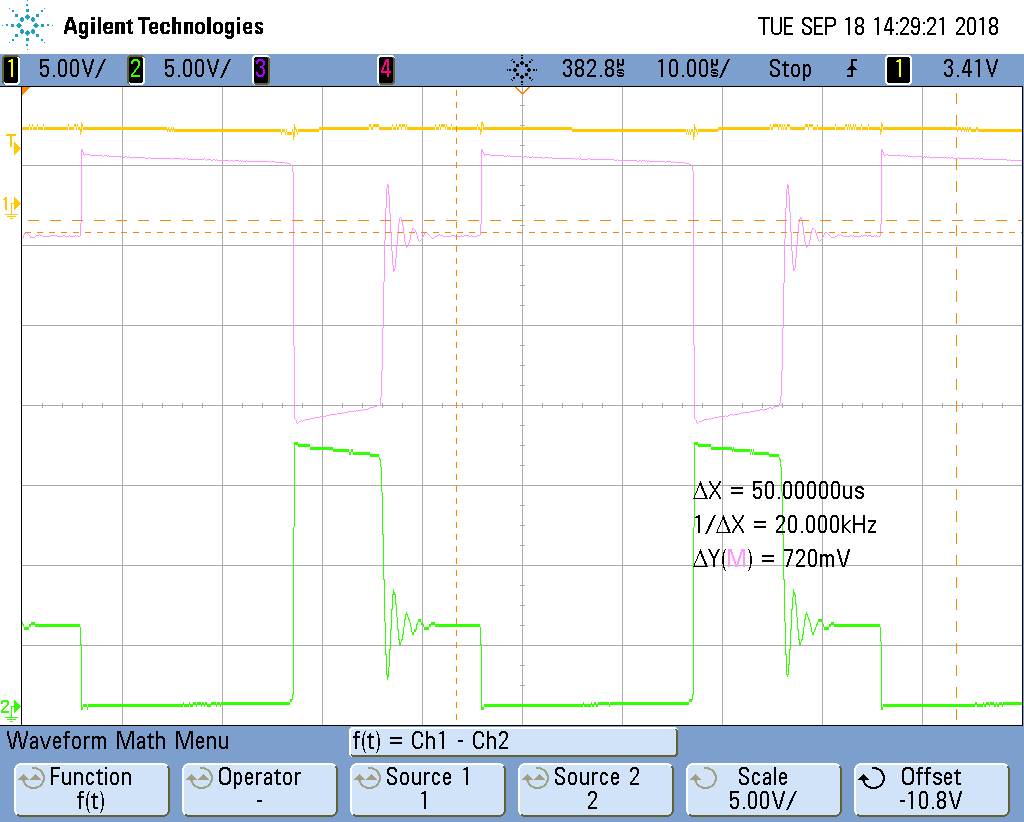
\includegraphics[width=0.9\textwidth]{Imagenes/vcoil.png}
\caption{Tensión sobre el inductor.}
	\label{fig:vcoil}
\end{figure}
Donde la señal rosa es la tensión sobre la bobina, la amarilla es la fuente y la verde sobre el otro nodo.
\begin{figure}[H]
	\centering
	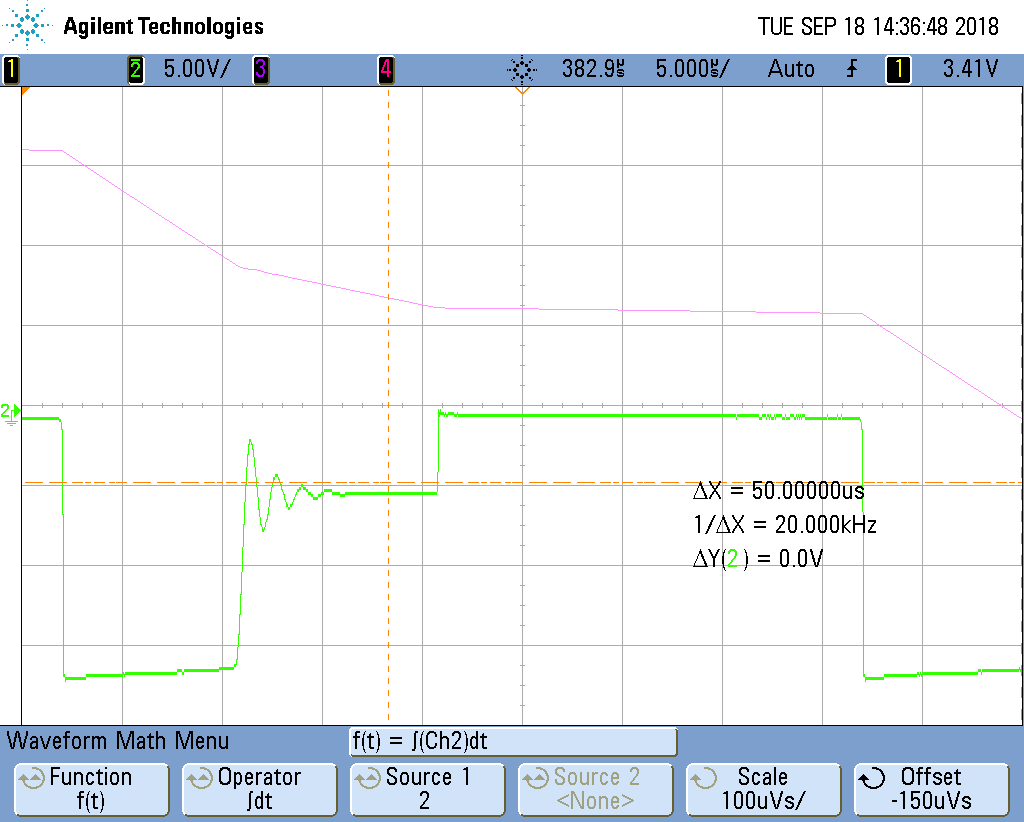
\includegraphics[width=0.9\textwidth]{Imagenes/icq_coil1.png}
\caption{Corriente sobre el inductor.}
	\label{fig:icoil}
\end{figure}
Donde la rosa es la corriente sobre el inductor y la verde es la tensión sobre el nodo de colector.
Para medir el valor de la inductancia se ideo la siguiente medición.
Se  propuso medir la inductancia como la razón entre la señal calculada por el osciloscopio\footnote{La cual es $I \cdot L = \int{V_{coil}}$} y la corriente que circula por la resistencia $R_L$.
Para que este resultado tena algún sentido fisico se propusieron las siguientes condiciones para la medición:
La medición se debe dar cuando el transistor esté en corte para que sea equivalente a un circuito abierto, y dado a que la entrada es una cuadrada, en ciertos intervalos se puede considerar el capacitor como un circuito abierto, por lo cual toda la corriente irá por la resistencia.
Se utilizó una frecuencia $f= 115kHz$ y un Duty-Cycle del 40\% .
Finalmente es de suma importancia que sean paralelas las señales a medir dado a que la medición se basa en la proporcionalidad de ambas corrientes por un factor "L".
\begin{figure}[H]
	\centering
	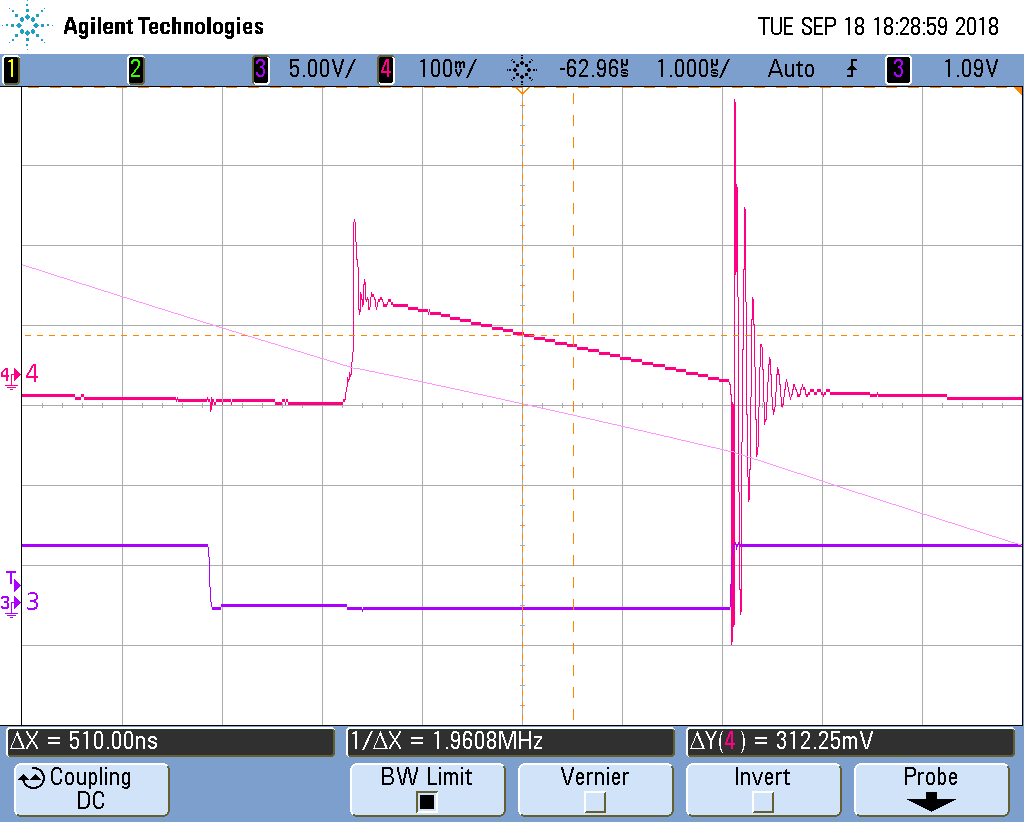
\includegraphics[width=0.9\textwidth]{Imagenes/mentira_para_.png}
\caption{Proporcionalidad de corrientes.}
	\label{fig:Lcoil}
\end{figure}
Donde la medición se hará en la zona donde son paralelas las señales, Siendo la roja la tensión sobre el resistor $R_L$ \footnote{La cual es proporcional a la corriente por un facot de 1K$\Omega$} y la rosa la corriente $I\cdot L$ calculada por el osciloscopio.\\
Fijando un tiempo $t_1$ se midió el cociente entre las corrientes para obtener la inductancia:
\begin{align} L = \frac{ L\cdot I(t_1)}{ I ( t_1)}\approx 512 \mu H \end{align}
el cual coincide aproximadamente con el valor nominal de la bobina

\begin{figure}[H]
\subfloat[]{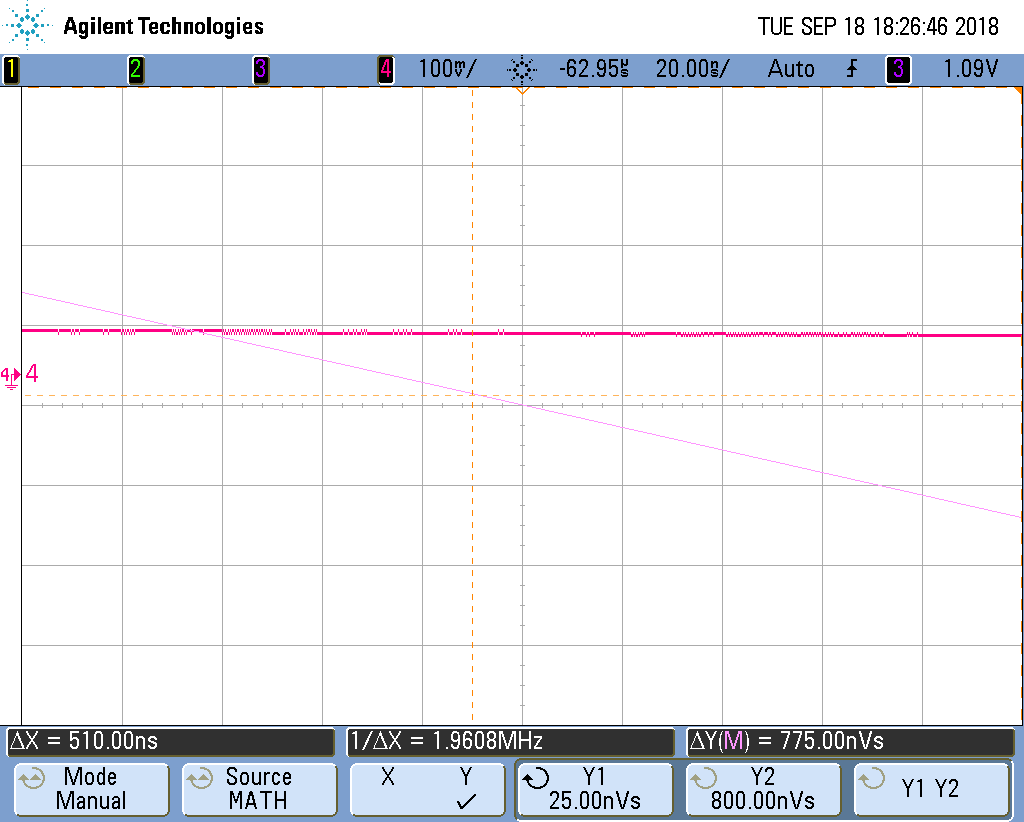
\includegraphics[width = 3in]{mentiraboth1.png}} 
\subfloat[]{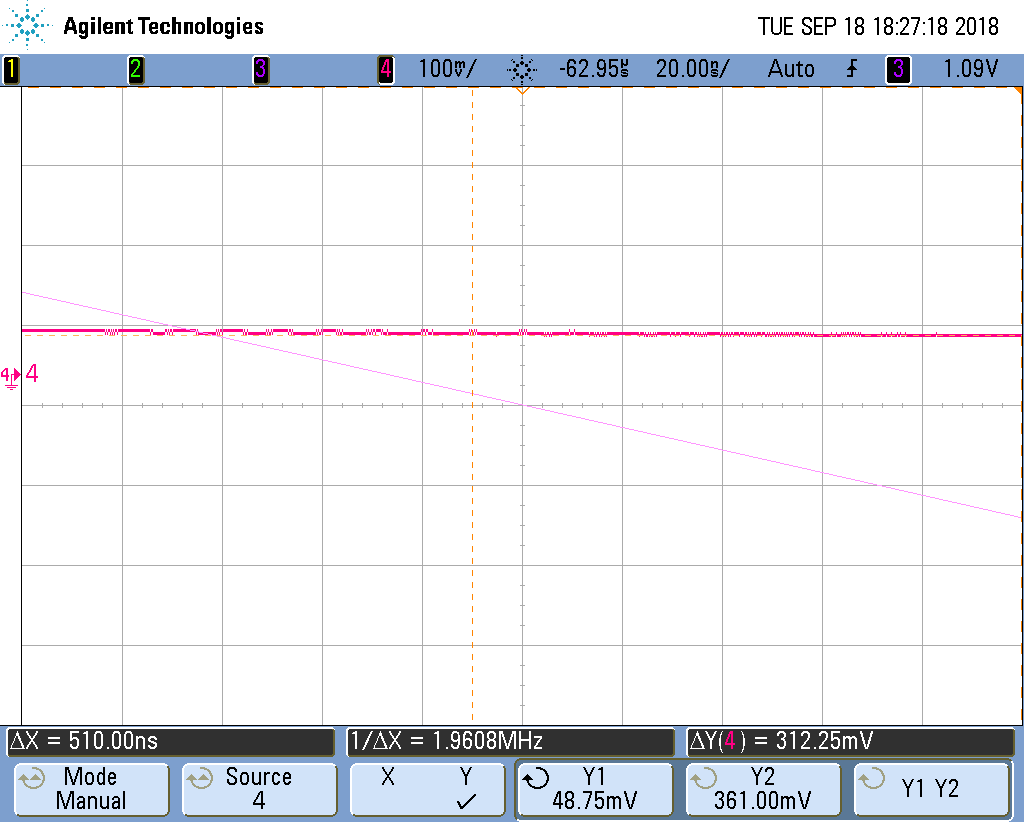
\includegraphics[width = 3in]{mentiraboth2.png}}\\
\caption{Medición del valor de la inductancia.}
\label{fig:medL}
\end{figure}
Luego se midió la tensión entre colector y base, obteniendo los siguientes resultados:
\begin{figure}[H]
	\centering
	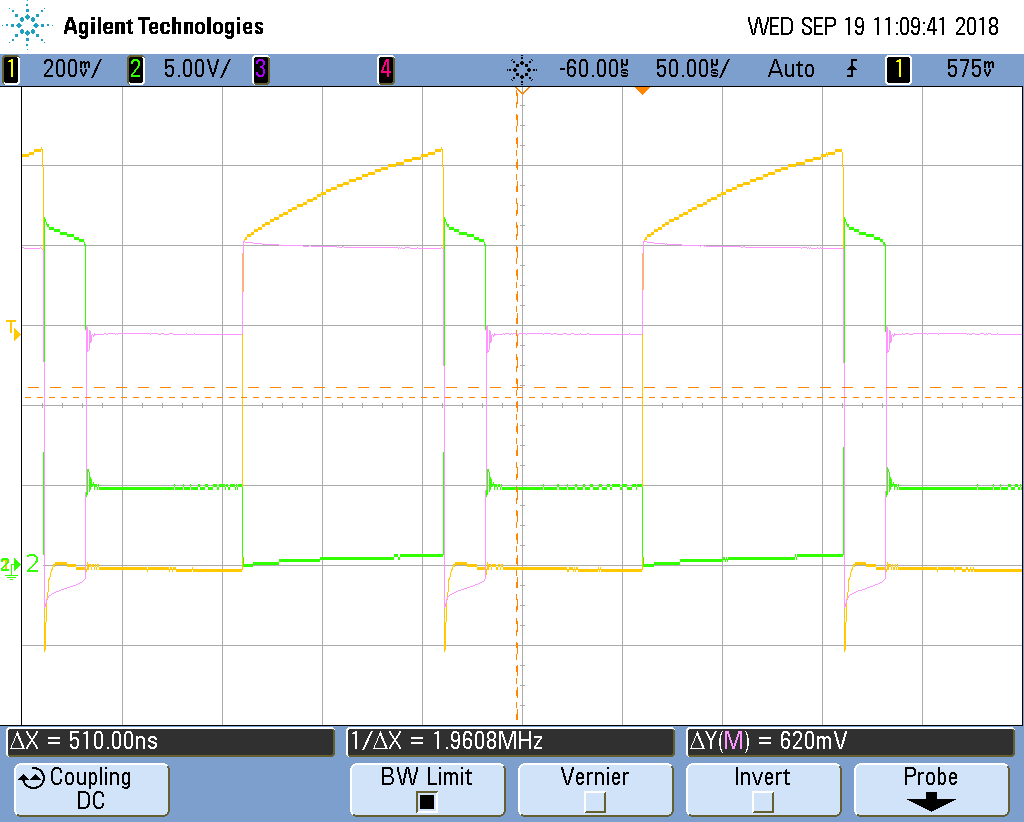
\includegraphics[width=0.9\textwidth]{Imagenes/vbc_vc_ab.png}
\caption{Tensión Base-Colector.}
	\label{fig:vbc}
\end{figure}
Donde la señal verde es la tensión en el colector, la amarilla la tensión en la base y finalmente la rosa es la tensión Base-Colector [Vb-Vc].
Se puede apreciar

Continuando, se midió la tension entre el colector y el emisor de distintas maneras. Utilizando el accesorio de resorte para la punta del osciloscopio, el cual permite no sumar a la medición la impedancia del cable de tierra y ademas la gran cercania en la adquisicion de la señal,  y además utilizando una punta con el cable de masa conectado directamente al cable de masa de la fuente de continua.obteniendo la siguiente imagen:
\begin{figure}[H]
	\centering
	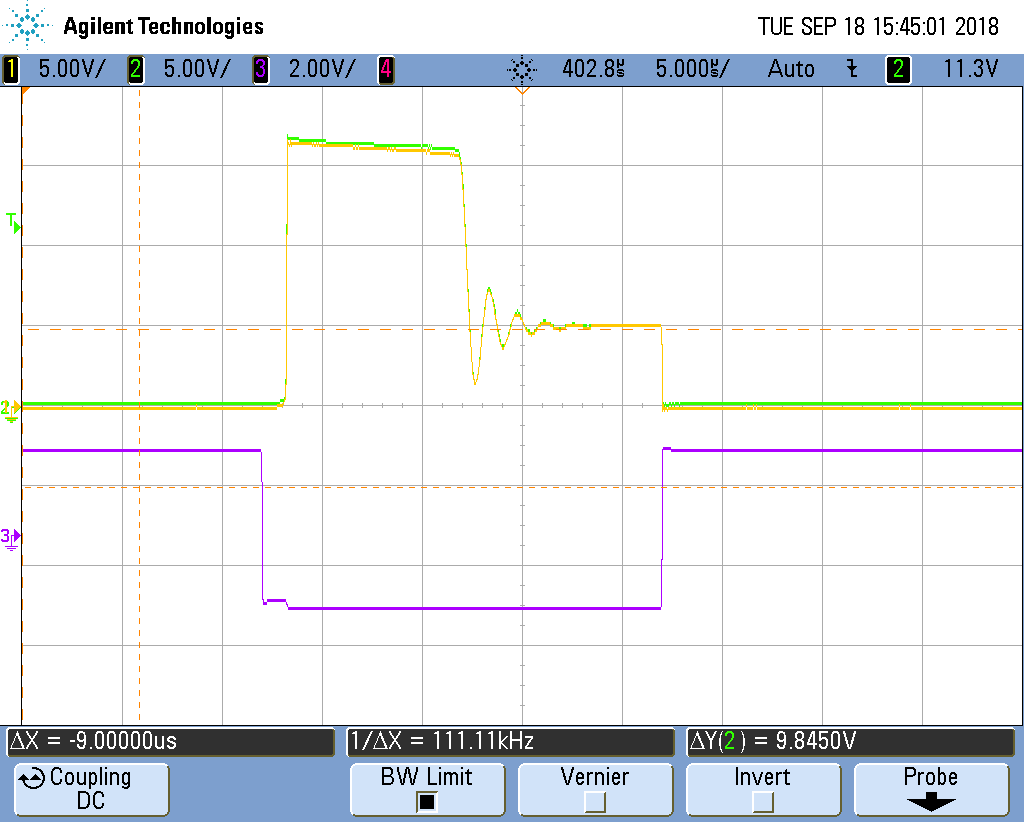
\includegraphics[width=0.9\textwidth]{Imagenes/vce_pe_both.png}
\caption{Tensión colector-emisor.}
	\label{fig:vce}
\end{figure}
Donde se puede apreciar como el transistor entra en la zona de corte, la cual es la zona con mayor tensión, y la zona de saturación donde la tensión se aproxima a cero, dado que en esas zonas el transistor se comporta tanto como un circuito abierto y un circuito cerrado respectivamente.\\Si bien no se nota una gran  diferencia  en la figura (\ref{fig:vce}) se debe a que estabamos en el momento utilizando el modo averaging del osciloscopio, luego se rehicieron las mediciones, utilizando únicamente el modo High-Resolution del osciloscopio y se notó que la medición realizada con el accesorio de resorte tenía menos ruido que la señal medida con el cable para su conección a tierra, esto se debe a que par el retorno de la señal a tierra el camino era mas directo. 

\end{document}
